% Cenário e troca de chaves.  TikZ puro, sem imagens externas.
\begin{figure}[!htb]
\centering
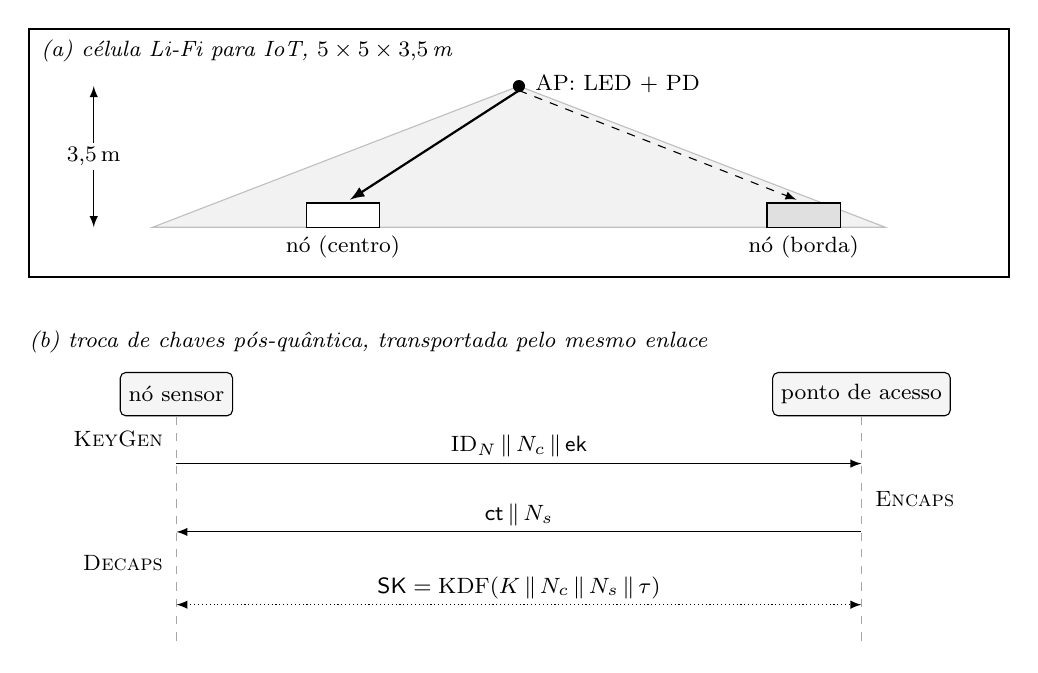
\begin{tikzpicture}[
  x=1.5cm, y=1.4cm,
  font=\footnotesize,
  box/.style={draw,rounded corners=2pt,align=center,inner sep=3pt,
              minimum height=5.5mm,fill=black!4},
  every path/.style={>=latex}
]
% ---------------------------- (a) sala ----------------------------
\begin{scope}
  \def\rw{8.3} \def\rh{2.25}
  \draw[thick] (0,0) rectangle (\rw,\rh);
  \node[anchor=north west,font=\footnotesize\itshape,inner sep=3pt]
       at (0.03,\rh-0.02) {(a) célula Li-Fi para IoT, $5\times5\times3{,}5$\,m};
  \draw[gray!50,fill=gray!10]
     (\rw/2,\rh-0.52) -- (1.05,0.45) -- (\rw-1.05,0.45) -- cycle;
  \fill (\rw/2,\rh-0.52) circle (2.2pt);
  \node[anchor=west,inner sep=4pt] at (\rw/2+0.04,\rh-0.50) {AP: LED $+$ PD};
  \draw[fill=white] (2.35,0.45) rectangle ++(0.62,0.22);
  \node[anchor=north,inner sep=3pt] at (2.66,0.45) {nó (centro)};
  \draw[fill=black!12] (6.25,0.45) rectangle ++(0.62,0.22);
  \node[anchor=north,inner sep=3pt] at (6.56,0.45) {nó (borda)};
  \draw[->,thick]  (\rw/2,\rh-0.56) -- (2.72,0.70);
  \draw[->,dashed] (\rw/2,\rh-0.56) -- (6.50,0.70);
  \draw[<->] (0.55,0.45) -- (0.55,\rh-0.52)
       node[midway,fill=white,inner sep=1.5pt] {$3{,}5$\,m};
\end{scope}
% ----------------------- (b) troca de chaves -----------------------
\begin{scope}[yshift=-4.5cm]
  \def\lx{1.25} \def\rx{7.05} \def\ty{2.15}
  \node[anchor=north west,font=\footnotesize\itshape,inner sep=0pt]
       at (0,\ty+0.58) {(b) troca de chaves pós-quântica, transportada pelo mesmo enlace};
  \node[box] (N) at (\lx,\ty) {nó sensor};
  \node[box] (A) at (\rx,\ty) {ponto de acesso};
  \draw[dashed,gray!70] (N) -- (\lx,-0.12);
  \draw[dashed,gray!70] (A) -- (\rx,-0.12);
  \draw[->] (\lx,1.52) -- node[above,inner sep=2pt]
      {$\mathrm{ID}_N \,\|\, N_c \,\|\, \mathsf{ek}$} (\rx,1.52);
  \node[anchor=east,inner sep=3pt] at (\lx-0.04,1.74)
      {\textsc{KeyGen}};
  \node[anchor=west,inner sep=3pt] at (\rx+0.04,1.20)
      {\textsc{Encaps}};
  \draw[<-] (\lx,0.90) -- node[above,inner sep=2pt]
      {$\mathsf{ct} \,\|\, N_s$} (\rx,0.90);
  \node[anchor=east,inner sep=3pt] at (\lx-0.04,0.62)
      {\textsc{Decaps}};
  \draw[<->,densely dotted] (\lx,0.24) --
      node[above,inner sep=2pt]
      {$\mathsf{SK}=\mathrm{KDF}(K \,\|\, N_c \,\|\, N_s \,\|\, \tau)$} (\rx,0.24);
\end{scope}
\end{tikzpicture}
\caption{O cenário estudado. (a) Um sensor sob a luminária e um sensor junto à
parede recebem quantidades de luz muito diferentes e, por isso, taxas de erro
muito diferentes. (b) A troca de chaves: o sensor envia a chave de
encapsulamento $\mathsf{ek}$, o ponto de acesso devolve o texto cifrado
$\mathsf{ct}$, e os dois derivam a chave de sessão $\mathsf{SK}$ pela
Eq.~\eqref{eq:kdf}.}
\label{fig:system}
\end{figure}
